
\chapter{Modelagem de sistemas não lineares}

A modelagem de sistemas não lineares pode ser feita de diversas formas, cada uma com vantagens e desvantagens próprias. As técnicas de modelagem não linear mais relevantes serão revisadas a seguir, apresentando um panorama geral de como elas funcionam e como são aplicadas.

\section*{\textit{Static Wave Shaping}}
\textit{Static Wave Shaping} significa modelagem estática de ondas. Esta técnica é consiste em aplicar um mapeamento da não linearidade do sistema relacionando a variável de entrada com uma variável de saída. A implementação dessa técnica se dá pela modelagem de equações que representam a não linearidade, como por exemplo:
\begin{equation}
y = \frac{3x}{2} (1 - \frac{{x^2}}{3})
\label{Equação1}
\end{equation}
Essa equação proposta por \cite{arayasuyama}  é implementada para se obter distorção de um sinal. A distorção se dá pela alimentação do sinal, que tem sua amplitude normalizada entre -1 e 1, na equação não linear através dos coeficientes de escala \cite{pakarinen2009review}. A função mostrada acima é descrita na imagem \ref{fig:staticwaveshaping}, onde ela apresenta uma certa linearidade para sinais pequenos de entrada e uma parte não linear quando se aproxima dos limites de x, entre -1 e 1.
\begin{figure}[htb!]
	\centering
	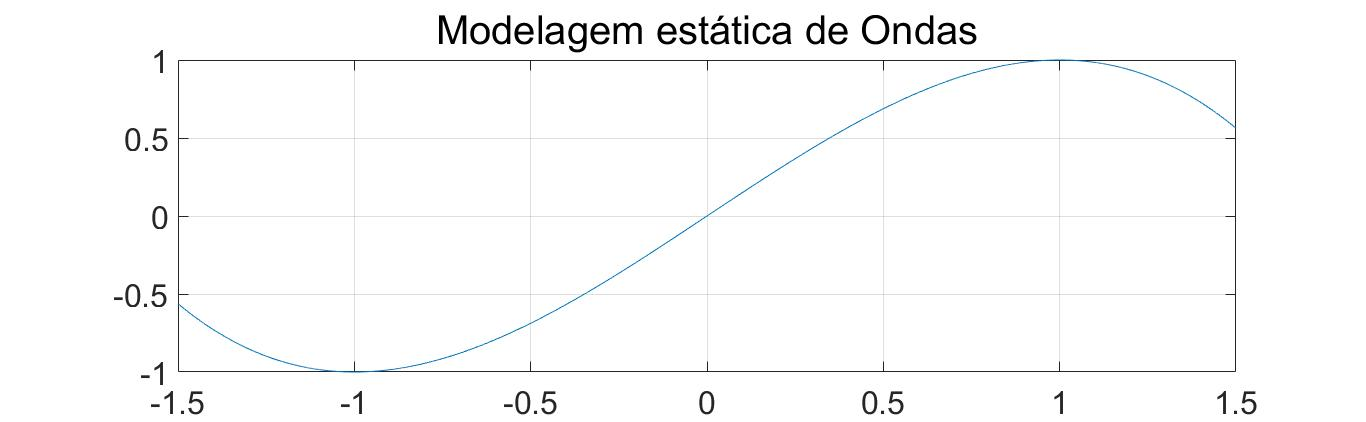
\includegraphics[width=0.7\linewidth]{figuras/StaticWaveShaping}
	\caption{Função não linear proposta por Araya e Suyama}
	\label{fig:staticwaveshaping}
\end{figure}

Um outro estudo realizado por \cite{moller2002measurement} apresenta um algorítimo para medir funções de transferências não lineares através de simulações utilizando o \textit{PSPICE}. O objetivo central do estudo era realizar uma mimica dos estágios de amplificação de um \textit{VOX AC 30}. Combinando simulações do esquemático elétrico do amplificador e exportando os dados obtidos para o \textit{MATLAB}.

\section*{\textit{Lookup Table Nonlinearity}}

A equação \ref{Equação1} pode ser também implementada através de uma técnica onde são pré computados os valores de saída para um valor determinado de entrada. A vantagem dessa técnica é a possibilidade de alterar os valores pré computados de maneira livre, sendo assim totalmente customizável\cite{pakarinen2009review}. A quantidade de dados que as tabelas contém está diretamente relacionada a resolução, ou seja, a qualidade e quantidade de detalhamento do som. Essa técnica foi utilizada pela Digidesign em um sintetizador que tinha como uma de suas funções, emular o som de uma guitarra distorcida. 

Estudos mais recentes realizados com \textit{Lookup Tables}
aproximam as tabelas com modelos \textit{Hammerstein}, que consistem em uma não linearidade estática, seguida por um filtro linear\cite{LUTFilter}. Esses modelos de \textit{Hammerstein} serão abordados mais detalhadamente posteriormente.

\section*{Análise nodal}
Através das Leis de Kirchhoff é possível obter o comportamento dos circuitos eletrônicos, utilizando modelos acurados dos componentes que compõem os amplificadores é possível relações aproximadas entre as tensões e as correntes que circulam pelo circuito \cite{pakarinen2009review}. Através de uma matriz de condutâncias, as tensões se relacionam com as correntes da seguinte forma:
\begin{equation}
Gv = \textit{c} 
\label{Equação2}
\end{equation}

Onde G na equação \ref{Equação2} é a matriz de condutâncias, \textit{v} é um vetor para cada voltagem no circuito e \textit{c} é o vetor que representa qualquer fonte de corrente em cada nó do circuito. Cada tipo de componente do circuito (resistor, capacitor, indutor, indutância mútua de transformadores,diodos, transistores) contribui com uma linha da matriz G. As correntes nas fontes de voltagem dependem de equações auxiliares que são adicionadas em colunas e linhas do sistema descrito acima. Esse método é chamado também de \textit{K-Method}, referindo-se as leis de Kirchhoff.
\begin{equation}
c=M_{1}x + M_{2}u + M_{3}i
\label{Equação3}
\end{equation}

Para aplicar o \textit{K-method}, a variável C na equação \ref{Equação2} é descrita pela equação \ref{Equação3}, onde é necessário escolher como as varáveis de estado \textbf{x}, as voltagens entre os capacitores e as correntes de indutores. A variável \textbf{u}, representa as fontes de corrente e voltagem presentes na entrada do circuito. Dispositivos não lineares contribuem com correntes não lineares \textbf{i} que são computadas por uma função vetorial \textbf{f} que mapeia as tensões controladas pelas correntes nos terminais dos dispositivos \cite{yeh2010automated1}. Como as correntes não lineares são dependentes das voltagens nos terminais de cada dispositivo não linear, a variável \textbf{i} é escrita em função de \textbf{v}. Então é possível modificar a equação \ref{Equação2} por:

\begin{equation}
Gv = M_{1}x + M_{2}u + M_{3}i(v) 
\label{Equação4}
\end{equation}

Essa técnica de modelagem, no entanto, depende da quantidade de nós que compõem o circuito para estimar o gasto computacional. Circuitos de amplificadores valvulados tendem a ser complexos e assim compromete a aplicação dessa técnica em tempo real.

\section*{\textit{Wave Digital Filters}}
\textit{Wave Digital Filters} são uma classe de filtros digitais onde é possível mapear seus parâmetros através das grandezas elétricas, como a tensão e a corrente. Cada elemento de um circuito elétrico possui uma representação em forma de filtro e através do uso de adaptadores é possível conectar diferentes filtros, como se fossem elementos de um circuito elétrico \cite{pakarinen2009review}. A construção de circuitos utilizando a técnica de \textit{Wave Digital Filters} se mostra eficiente e promissora para aplicações em tempo real, apesar de existirem algumas barreiras e topologias que não são mapeadas facilmente pela técnica.

O princípio por trás de \textit{Wave Digital Filters} é a transformação das variáveis de \textit{Kirchhoff}, tensão \textbf{v} e corrente \textbf{i}, em parâmetros utilizados na criação dos filtros, chamados de variáveis de onda (reflectância e incidência) \cite{2012Macak}.

A figura \ref{fig:componentesemwdf} resume as transformações para cada componente básico de um circuito.
\begin{figure}[!htb]
	\centering
	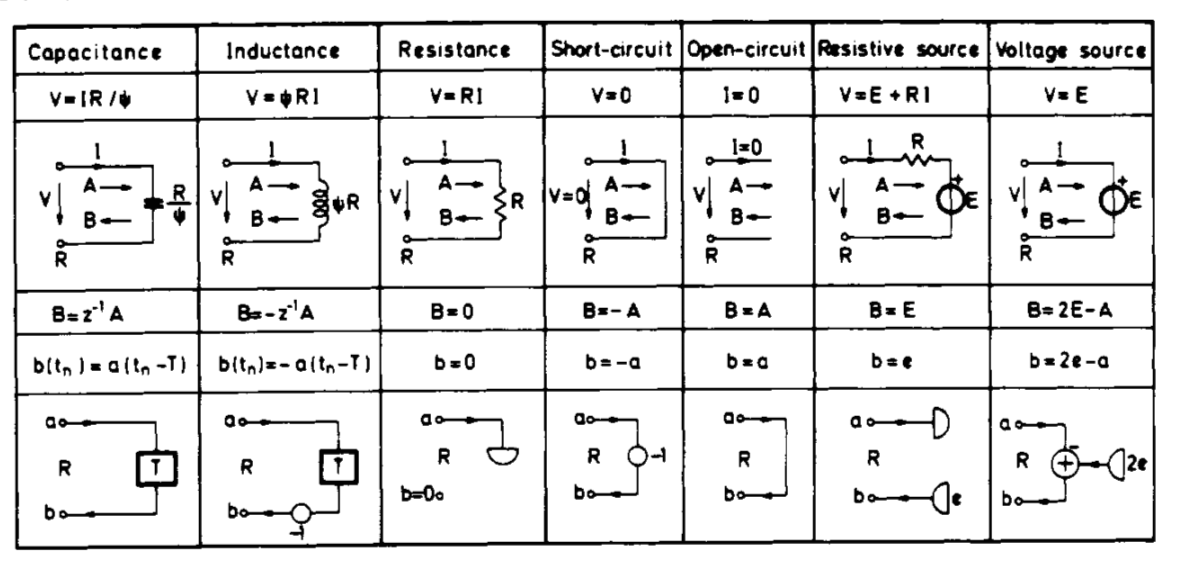
\includegraphics[width=0.7\linewidth]{figuras/ComponentesemWDF}
	\caption{Elementos básicos de um circuito e suas representações em grandezas de onda. Autor \cite{fettweis1986wave}.}
	\label{fig:componentesemwdf}
\end{figure}




\section*{Séries de Volterra}{\label{Volterra}}
É um método analítico que usa uma ferramenta matemática chamada séries de Volterra para modelar um sistema não linear. Série de Volterra é, por definição, uma convolução multidimensional da entrada do sistema com uma matriz de resposta não linear. Enquanto a resposta ao impulso em sistemas lineares caracteriza por completo um sistema e permite prever uma resposta para uma determinada entrada, em sistemas não lineares, esse tipo de caracterização não consegue identificar as não linearidades, caracterizando assim somente a parte linear do sistema. As Séries de Volterra permitem caracterizar, através de funções especiais, chamadas de \textit{kernels}, a parte não linear do sistema. Os \kernels correspondem a resposta multidimensional ao impulso dos coeficientes não lineares do sistema. \cite{pakarinen2009review}

As séries de Volterra podem ser consideradas também como uma expansão em séries de Taylor com os coeficientes do polinômio substituídos por convoluções multidimensionais representando assim o efeito de memória de sistemas não lineares de acordo com a ordem de não linearidade \cite{pakarinen2009review}



\subsection*{Definição no domínio do tempo}
Em sistemas lineares a convolução é representada por:
\begin{equation}
y(t) = \int_{-\infty}^{\infty} h(t-\tau)x(\tau)d\tau = h(t)*x(t)
\label{Integral de convolução}
\end{equation}
Onde $x(t)$ é a entrada do sistema, $y(t)$ é a saída e $h(t)$ é a resposta ao impulso do sistema. Aplicando a transformada de Fourier tem-se que:

\begin{equation}
Y(j\omega) = H(j\omega)X(j\omega)
\label{Equação 3.2}
\end{equation}

Assim, a resposta ao impulso $h(t)$ na equação \ref{Integral de convolução} e a resposta em frequência $H(j\omega)$ em \ref{Equação 3.2} contém toda a informação necessária para se caracterizar um sistema \cite{cheng2017volterra}

Para sistemas não lineares, se a energia contida no sinal $x(t)$ é limitada, significa que o sinal pode ser representado por Séries de Volterra.

\begin{equation}
y(t)=h_{0} + \sum_{n=1}^{N} \int_{a}^{b}\cdot\cdot\cdot\int_{a}^{b} h_{n}(\tau_{1},...,\tau_{n})\prod_{j=1}^{n}x(t - \tau_{j})d\tau_{j}
\label{Equação de Volterra}
\end{equation}

Os coeficientes $h_{n}$ são os \textit{kernels}. O termo $h_{0}$ é chamado de constante de ordem zero. É interessante notar que se todos os \textit{kernels}, exceto o de primeira ordem, forem iguais a zero, o sistema em análise é puramente linear.



\subsection*{Definição no Domínio Discreto}
Na maioria das vezes, utiliza-se computadores para realizar os cálculos das séries de Volterra. Devido a complexidade dos sistemas não lineares, facilmente os cálculos se tornam inviáveis de serem realizados analiticamente. Para que o computador possa realizar os cálculos é necessário uma representação discreta da série de Volterra

As séries de Volterra em tempo discreto são definidas como:
\begin{equation}
y[n] = h_{0} + \sum_{p=1}^{P}\sum_{\tau_{1} = a}^{b}\dots\sum_{\tau_{p}= a}^{b} h_{p}(\tau_{1},\dots,\tau_{p}) \prod_{j = 1}^{p} x(n - \tau_{j})
\label{Equação 3.4}
\end{equation}

Essa equação é capaz de descrever sistemas não lineares com memória e sua implementação computacional se dá por um método bem simples e direto através de um algorítimo que represente os somatórios mostrados na equação \ref{Equação 3.4}.


\section*{Domínio da frequência}
Para sistemas lineares, a resposta em frequência facilita bastante a análise e modelagem de sistemas. Infelizmente para os não lineares a resposta em frequência não ajuda na análise nem na modelagem. Para isso, desenvolveu-se, baseado em Séries de Volterra, alguns conceitos para se analisar sistemas não lineares no domínio da frequência. Conceitos como Função de Resposta em Frequência Generalizada, Função da Resposta em Frequência Não Linear da Saída entre outras que serão apresentadas a seguir:
\subsubsection*{Função de Resposta em Frequência Generalizada }
A \FRFG, também conhecida como \textit{Generalized frequency response function (GFRF)} em inglês, é definida como a Transformada de Fourier multidimensional dos \kernels de Volterra e pode ser representada por:

\begin{equation}
H_{n}(\omega_{1},...,\omega_{n}) = \int_{- \infty}^{\infty}\cdots \int_{- \infty}^{\infty}h_{n}(\tau_{1},\cdots,\tau_{n})e^{-j(\omega_{1}\tau_{1}+\cdots+\omega_{n}\tau_{n})}d\tau_{1}\cdots d\tau_{n}
\label{Equação 3.8}
\end{equation}

A transformada inversa pode ser feita como:
\begin{equation}
h_{n}(\tau_{1},...,\tau_{n}) = \dfrac{1}{(2\pi)^{n}}\int_{- \infty}^{\infty}\cdots \int_{- \infty}^{\infty}H_{n}(\omega_{1},\cdots,\omega_{n})e^{j(\omega_{1}\tau_{1}+\cdots+\omega_{n}\tau_{n})}d\omega_{1}\cdots d\omega_{n}
\label{Equação 3.9}
\end{equation}

Usando a \FRFG tem-se que a saída de um sistema não linear é representada no domínio da frequência como:

\begin{equation}
Y(\omega) = \sum_{n=1}^{\infty} Y_{n}(\omega)
\label{Equação 3.11}
\end{equation}

Onde, $Y_{n}(\omega)$ é:
\begin{equation}
Y_{n}(\omega) = \dfrac{\frac{1}{\sqrt{n}}}{(2 \pi)^{n-1}}\int_{\omega_{1},\cdots,\omega_{n}=\omega}H_{n}(\omega_{1},\cdots,\omega)\prod_{i=1}^{n}U(\omega_{i}) d\sigma_{n\omega}
\label{Equação 3.12}
\end{equation}

Para as equações \ref{Equação 3.12} e \ref{Equação 3.11}, $Y(\omega)$é todo o espectro da saída do sistema, $U(\omega)$ é o espectro da entrada do sistema, $Y_{n}(\omega)$ representa a n-ésima ordem da resposta em frequência da saída do sistema, $\sigma_{n\omega}$ representa todo o campo de integração satisfazendo a restrição $\omega_{1},\cdots,\omega_{n}=\omega$.

Em sistemas lineares, a função da resposta em frequência pode ser deduzida utilizando a transformada de Laplace, através das equações diferenciais dinâmicas \cite{cheng2017volterra}. \cite{bedrosian1971output} propôs um método de análise dos harmônicos gerados por distorções em sistemas de comunicação, porém o método de análise proposto só é válido para sistemas de uma única entrada. Vários outros estudos buscaram extender as pesquisas de \cite{bedrosian1971output} para múltiplas entradas como as pesquisas de \cite{Swain} e \cite{HeFei}.

\subsubsection*{Função da Resposta em Frequência não linear da Saida }
Uma das principais características da \FRFG é que ela é multidimensional. A quantidade de dimensões presentes em um sistema torna a função muito mais complicada de se medir, mostrar e interpretar do que a resposta em frequência de um sistema linear. Para isso foi proposto uma função de uma dimensão na frequência que permite uma análise de sistemas não lineares de forma semelhante a sistemas lineares. A NOFRF (\textit{Nonlinear output frequency response function}) é definida como:

\begin{equation}
G_{n}(\omega) = \dfrac{\int_{\omega_{1}+\cdots+\omega_{n}=\omega}H_{n}(\omega_{1},\cdots,\omega_{n})\prod_{i=1}^{n}U(\omega_{i})d\sigma_{n\omega} }{\int_{\omega_{1}+\cdots+\omega_{n}=\omega}\prod_{i=1}^{n}U(\omega_{i})d\sigma_{n\omega}}
\label{Equação 3.13}
\end{equation}

Sob a condição que:
$$U_{n}(\omega) = \int_{\omega_{1}+\cdots+\omega_{n}=\omega}\prod_{i=1}^{n}U(\omega_{i})d\sigma_{n\omega} \neq 0$$

Sendo assim a resposta em frequência do sistema, pelo conceito introduzido pela NOFRF é dada por:

\begin{equation}
Y(\omega) = \sum_{n=1}^{N} Y_{n}(\omega) = \sum_{n=1}^{N} G_{n}(\omega) U_{n}(\omega)
\label{Equação 3.14}
\end{equation} 

A variável $U_{n}(\omega)$ é definida da mesma forma como é mostrada na equação \ref{Equação 3.13}. A grande vantagem da NOFRF é representar um sistema em uma única dimensão. É importante perceber que a NOFRF não está relacionada somente a as características do sistema, mas também está relacionada a entrada do sistema, refletindo em uma contribuição combinada entre o sistema e a entrada do sistema com o comportamento da resposta em frequência da saída do sistema \cite{cheng2017volterra}.	

\subsection*{Relação entre as Séries de Volterra e outros modelos não lineares}
Existem várias relações que aproximam as Séries de Volterra com modelos de sistemas não lineares como as séries de Taylor, séries de Wiener, modelos de Hammerstein, Wiener-Hammerstein e outros mais.

\subsubsection*{Séries de Taylor}
É um dos métodos mais típicos para se descrever a realação não linear entre duas variáveis. Assumindo que a relação entre duas variáveis $y$ e $u$ pode ser decrita pela função $y = f(u)$. Se a função $f$ no ponto $u_{0}$ é infitamente diferenciável, então nos limites de $u_{0}$, a variável $y$ pode ser expressa como uma série de potências da variável $u$. Especialmente quando $u_{0} = 0$ as séries de Taylor são denominadas Séries de Maclaurin e são representadas da seguinte forma\cite{cheng2017volterra}:

\begin{equation}
y = f(0) + f^{'}(0)u + \dfrac{f^{''}(0)}{2!}u^{2}+\cdots+\dfrac{f^{(n)}(0)}{n!}u^{n}+\cdots$$
$$ y =\sum_{i=0}^{\infty} \dfrac{f^{(i)}(0)}{i!}u^{i}
\label{Equação 4.15}
\end{equation}

De acordo com a definição das Séries de Volterra, a função dos \kernels da série é a função delta de Dirac multidimensional e pode ser escrita como:

\begin{equation}
h_{n}(\tau_{1},\cdots,\tau_{n})=a_{n}\delta(\tau_{1})\cdots\delta(\tau_{n})
\label{Equação 4.16}
\end{equation}
A equação \ref{Equação de Volterra} pode ser reescrita como:

\begin{equation}
y(t) = \int_{-\infty}^{\infty} \cdots \int_{-\infty}^{\infty} a_{n}\delta(\tau_{1})\cdots\delta(\tau_{n}\prod_{j=1}^{n}x(\tau - \tau_{j})d\tau1 \cdots d\tau_{n}$$
$$ y(t) = \sum_{n=1}^{\infty} a_{n}x^{n}(t)
\end{equation}

Neste caso a série de Volterra se degenera em uma série ordinária, similar a série de Taylor. O atraso $\tau_{j}$ representa o efeito da entrada atual e da entrada passada na saída presente. Se os \kernels forem escolhidos da mesma forma como a equação \ref{Equação 4.16}, significa que somente quando todos os atrasos $\tau_{j} = 0$ a função dos \kernels seria diferente de 0. Isso implica que entradas passadas não podem afetar a resposta atual do sistema. O fato das séries de Volterra levar em consideração diferentes atrasos faz ela ser uma extensão das séries de Taylor que leva em consideração efeitos de memória e a dinâmica do sistema, enquanto as séries de taylor so conseguem representar a não linearidade estática do sistema \cite{cheng2017volterra}.

\subsubsection*{Séries de Wiener}
Em alguns casos as séries de Volterra apresentam algumas disvantagens na analise e modelagem de sistemas não lineares. A região de convergência é bem estreita, e a identificação do \kernels é uma tarefa difícil. Para evitar a difícil convergência das séries de Volterra, as séries de Wiener é essencialmente a expansão ortogonal de séries de funções para sistemas não lineares invariantes no tempo e possuem uma relação próxima com as séries de Volterra. Dado que a representação da série Wiener é conhecida, então cada ordem da série Volterra pode ser derivada adicionando cada ordem da série Wiener.
Dado que a representação da série de Volterra é conhecida, então cada ordem da série de Wiener pode ser obtida aplicando o procedimento de ortogonalização de Gram-Schmid.

\begin{equation}
\left\{\begin{array}{ll}y(t) = G_{0} + \sum_{n = 1}^{\infty} G_{n}[x(t)]\\G_{n}[x(t)] = G_{0,n} + G_{1,n}[x(t)]+ \cdots + G_{n,n}[x(t)]\end{array}\right.
\label{Equação 4.18}
\end{equation}

Onde $x(t)$ é a entrada, $G_{0}$ é a componente de ordem zero, $G_{n}[x(t)]$ é a enésima componente $G$ que é constituída pela enésima ordem da série não homogênea de Volterra, e $G_{r,n}(\tau_{1},\cdots,\tau_{r})(r \leq n)$ pode ser representado como:

\begin{equation}
G_{r,n}[x(t)] = \int_{0}^{\infty} \cdots \int_{0}^{\infty} G_{r,n}(\tau_{1},\cdots,\tau_{r})x(t-\tau_{1})\cdots x(t - \tau_{r})d\tau_{1}\cdots d\tau_{r}
\label{Equação 4.19}
\end{equation}

Onde $G_{r,n}(\tau_{1},\cdots,\tau_{r})(r \leq n)$ na equação \ref{Equação 4.19} é a função dos \kernels de Wiener.

Sendo que cada ordem de G é mutualmente ortogonal, podendo ser expressa como:
\begin{equation}
E(G_{n}[x(t)]G_{m}[x(t)]) = 0$$
$$n \neq m 
\end{equation}


Um método de identificação direta dos \kernels de Wiener foi proposto por Lee e Schetzen em \cite{lee1965measurement}.

\begin{equation}
G_{n,n}(\tau_{1},\cdots,\tau_{n}) = \dfrac{1}{x! \sigma_{x}^{2n}}  \overline{( y(t) - \sum_{i = 1}^{n -1}G_{i}[x(t)]) x(t-\tau_{1} \cdots x(t-\tau_{n}))}
\end{equation}

Onde a barra indica a média sobre o tempo e $\sigma_{x}^{2}$ é variância da entrada.



\subsubsection*{Modelo de Hammerstein}
O modelo de \textit{Hammerstein} é constituído por um subsistema não linear estático seguido por um subsistema linear e pode ser modelado como:
\begin{equation}
y = \int_{- \infty}^{\infty}h(\tau) x(t-\tau) d\tau
\label{Equação 4.23}
\end{equation}
\begin{equation}
x(t)=F(u(t))
\label{Equação 4.24}
\end{equation}
Onde $u(t)$ é a entrada do sistema, $y(t)$ é a saída e $F(.)$ é a função não linear. De acordo com as equações \ref{Equação 4.23} e \ref{Equação 4.24}, a relação entre a entrada e a saída do sistema é dada por:
\begin{equation}
y(t) = \int_{-\infty}^{\infty} h(\tau) \sum_{n=1}^{N}a_{n}[u(t-\tau)]^{n}d\tau =$$
$$ \sum_{n=1}^{N} \int_{-\infty}^{\infty}a_{n}h(\tau)[u(t-\tau)]^{n}d\tau =$$
$$ y(t) = \sum_{n=1}^{N} y_{n}(t)
\label{Equção 4.25}
\end{equation}

Onde,
\begin{equation}
y_{n}(t) =  \int_{-\infty}^{\infty} \cdots \int_{-\infty}^{\infty}  (a_{n}h(\tau_{1})\sigma(\tau_{1} - \tau_{2}) \cdots \sigma(\tau_{1} - \tau_{n})/[\Delta\tau]^{n-1}) u(t-\tau_{n})\cdots u(t-\tau_{n})d\tau_{1}\cdots d\tau_{n}
\label{Equação 4.26}
\end{equation}

O modelo de Hammerstein então é uma série de Volterra truncada com as funções de \kernels sendo:

\begin{equation}
h_{n}(\tau_{1},\cdots,\tau_{n})=a_{n}h(\tau_{1})\sigma(\tau_{1} - \tau_{2}) \cdots \sigma(\tau_{1} - \tau_{n})/[\Delta\tau]^{n-1} $$
$$ = a_{n}h(\tau)/[\Delta\tau]^{n-1}
\end{equation}

ou 
\begin{equation}
h_{n}(\tau_{1},\cdots,\tau_{n}) = \left\{\begin{array}{ll} 0  , \tau_{1} \neq \tau_{n}\\ a_{n}h(\tau_{1})\sigma(\tau_{1} - \tau_{2}) \cdots \sigma(\tau_{1} - \tau_{n})/[\Delta \tau]^{n-1} , \tau_{1} = \tau_{n} \end{array}\right.
\label{Equação 4.28}
\end{equation}

A equação \ref{Equação 4.28} mostra que somente os \kernels que formam a diagonal principal de uma matriz de \kernels são diferentes de zero.\cite{cheng2017volterra}

\subsection*{Convergência das Séries de Volterra}
Para identificar se as séries de Volterra são convergentes é necessário levar em conta dois aspectos. O primeiro aspecto é analisar se a série é convergente e o segundo é se a representação da série é convergente. A solução do primeiro aspecto define se o sistema pode ser aproximado por séries de Volterra. A convergência média quadrática é definida como: dada uma sequência de variáveis $X_{1}, X_{2},X_{3},\cdots$ que converge para uma variável $X$ em média quadrática é:

\begin{equation}
\lim\limits_{n \rightarrow \infty} E[(X_{n} - X)^{2}] = 0
\end{equation} 
Onde $E[X]$ é a média finita.

Se a convergência média quadrática da saída do sistema e do modelo for selecionada, as classes mais gerais de sistemas podem ser recuperados. Neste caso, efeitos não lineares como descontinuidades e saturação podem ser modelada por séries de Volterra. Escolhendo a convergência uniforme, somente a saturação não linear pode ser modelada. A solução do segundo aspecto pode ser usada para analisar a precisão da aproximação, a ordem de truncamento da série pode ser escolhida de acordo com o requisito de precisão de aproximação. A ideia básica para achar a região de convergência é procurar uma região de convergência de séries de potência que seja mais restritiva que a região de convergência das séries de Volterra.

Supondo que para todo o tempo
$|u(t)| < K$ e $$\int_{-\infty}^{\infty} \cdots\int_{-\infty}^{\infty} |h_{n}(\tau_{1},\cdots,\tau_{n})| d\tau_{1}\cdots d\tau_{n} \leq a_{n}$$

de acordo com a definição da série de Volterra, a saída do sistema segue a equação a seguir:

\begin{equation}
|y(t)| \leq \sum_{n = 0}^{\infty}a_{n}K^{n}
\label{Equação 4.29}
\end{equation}

Caso a série de potência do lado direito da equação \ref{Equação 4.29} seja convergente então a série de Volterra também será.

\section*{A identificação dos \kernels de Volterra} \label{ident}
Um dos principais problemas para a modelagem de sistemas usando as séries de Volterra é a identificação dos \kernels que caracterizam a série. Para identificar os núcleos é necessário excitar o amplificador a ser modelado com um sinal que consiga saturar as válvulas de tal forma que ocorra a distorção do amplificador. Proposto por Farina em \cite{farina2001non}, a aplicação de um sinal senoidal exponencial que varre a frequência audível (\textit{Swept Sines}) em um amplificador é capaz de extrair os núcleos da série e assim, é possível separar a resposta a cada harmônico do amplificador \cite{schmitz2017hammerstein}. Algumas modificações foram propostas ao modelo de Farina, corrigindo a formulação do sinal e evitando uma divergência entre as fases dos sinais \cite{novakdissertation}.

\textit{Swept Sines} são sinais senoidais que com o passar do tempo variam a sua frequência instantânea, cobrindo uma faixa do espectro de frequências.
São muito usados na área de comunicação em sonares e radares, mas também podem ser utilizado em sistemas de áudio para cobrir toda a frequência audível.

Um sinal desse tipo que aumenta a sua frequência exponencialmente é definido como:
\begin{equation}
x(t) = sin (2\pi f_{1}L [exp(\dfrac{t}{L})])
\label{sinal exponencial}
\end{equation}

Onde, a frequência instantânea é dada por:
\begin{equation}
f_{i}(t) = f_{1} exp(\dfrac{t}{L})
\end{equation}

o atraso de grupo $t_{f}$ é a função inversa da frequência instantânea $f_{i}$ e é dada por:
\begin{equation}
t_{f}(f) = L \ln(\dfrac{f_{i}}{f_{1}})
\end{equation}

A duração de tempo $T$ do sinal $x(t)$ pode ser expressa em função da frequência $f_{1}$ e da frequência $f_{2}$ que são, respectivamente, a frequência em que o sinal começa e a frequência em que o sinal termina\cite{novak2010nonlinear}.

\begin{equation}
T = L \ln(\dfrac{f_{2}}{f_{1}})
\label{Equação 5.10}
\end{equation}

A imagem abaixo mostra como a frequência do sinal varia com o passar do tempo.
\begin{figure}[!htb]
	\centering
	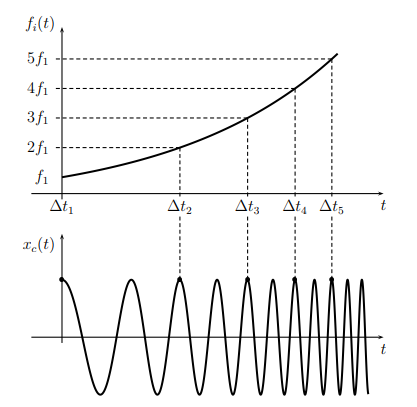
\includegraphics[width=0.5\linewidth]{figuras/SSS}
	\caption{Em cima: Frequência instantânea $f_{i}$. Embaixo: \textit{swept signal} sincronizado. Autor: \cite{novak2010chebyshev}}
	\label{fig:sss}
\end{figure}
